\section{Darlington circuit}
The circuit given in Figure 9.1 is known as a darlington circuit. Calculate \(I_{BE} , I_{AC} , I_{AL}\),
and the overall current gain \(\frac{I_{AL}}{I_{BE}}\). After that, simulate the circuit to double-check your
theoretical calculations. Assume both transistors have the same current gain coefficient
\(\beta = 100.\)
\begin{figure}[ht]
    \centering
    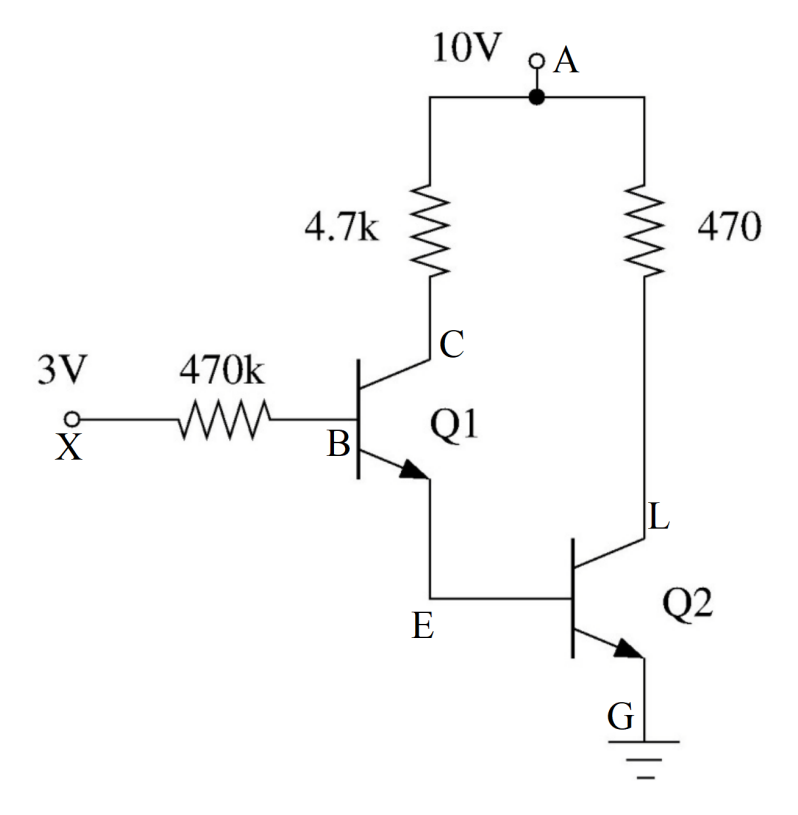
\includegraphics[scale=0.4]{graphics/ex9/f1.png}
    \caption{Darlington circuit}
\end{figure}
\subsection{Tính toán lý thuyết}
\textbf{Ghi chú:}

Những giải thích, công thức và phương trình được mong đợi hơn là chỉ có kết quả.

Giả sử BJT \(Q_1\) và \(Q_2\) trong vùng tích cực: \(V_{BE} \approx 0,7 \) V và \(V_{EG} \approx 0,7\) V
    \begin{align*}
    &I_{BE}=\dfrac{V_X - V_{BE} - V_{EG}}{470.10^3} = \dfrac{3 - 0,7 - 0,7}{470.10^3} \approx 3,4 (\mu A) \\
    &I_{AC} = \beta I_{BE} = 100.3,4 = 0,34 (mA)\\
    &I_{AL} = \beta I_{EG} = 100.(I_{AC} + I_{BE}) = 100.(0,34.10^{-3} + 3,4.10^{-6}) = 34,34 (mA)\\
    &\dfrac{I_{AL}}{I_{BE}} = \dfrac{34,34.10^{-3}}{3,4.10^{-6}} = 10100\\
    \end{align*}
    \newpage
\subsection{Mô phỏng}
\begin{figure}[ht]
    \centering
    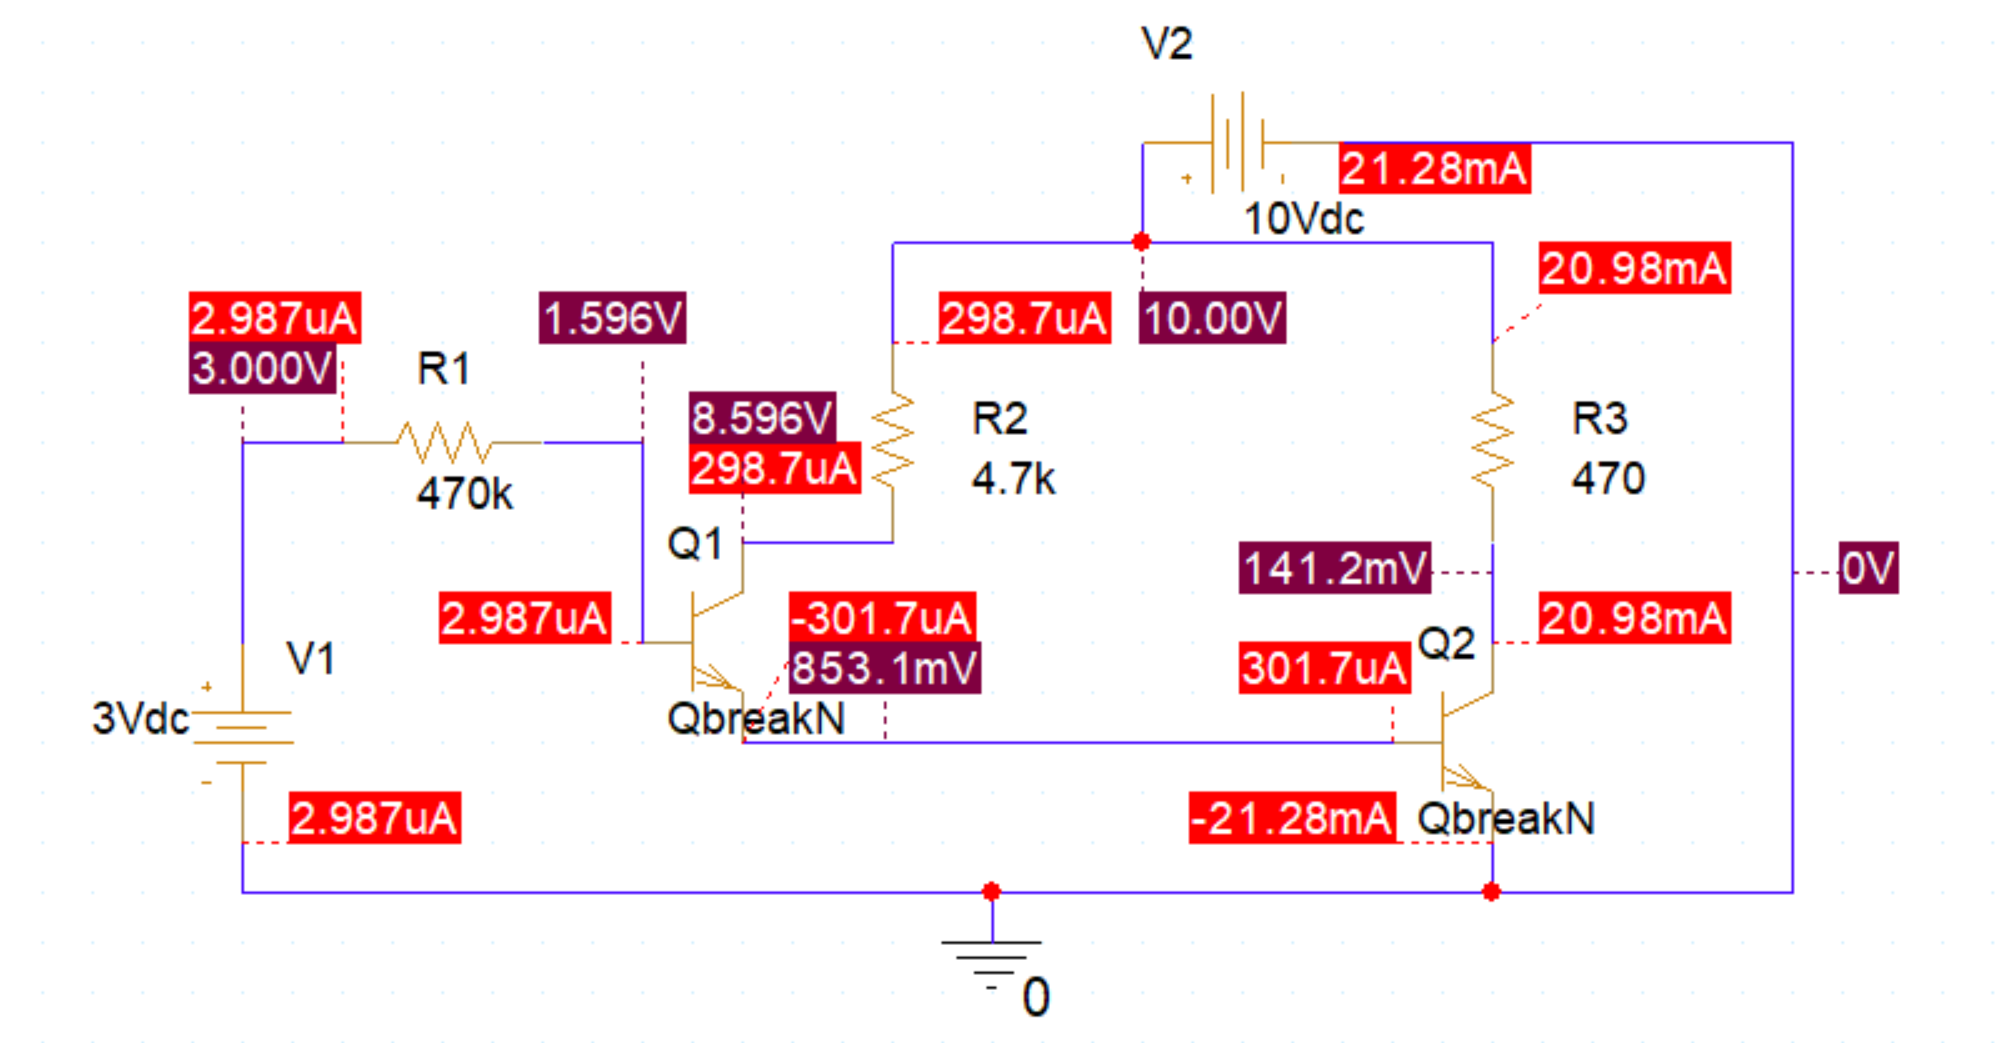
\includegraphics[scale=0.3]{graphics/ex9/f2.png}
    \caption{Darlington circuit}
\end{figure}

Do ta giả sử \(V_{BE} \approx 0,7 \) V và \(V_{EG} \approx 0,7 \) V trong khi mô phỏng \(V_{BE} \approx 0,799 \) V và \(V_{EG} \approx 0,799 \) V nên kết quả mô phỏng có sự trên lệch so với tính toán lí thuyết.

\pagebreak